\subsubsection{Control}
\begin{figure}[H]
\centering
\includegraphics[width = 1.0  \textwidth]{Figurer/classesControl.pdf}
\caption{Klassediagram over de klasser der er med i Control-delen af MVC designmønstret.}
\label{fig:classesControl}
\end{figure}
%   RR
%    \item Hvordan og hvornår opdateres modellen? 
\textbf{Opdatering af modellen:} 
Det er valgt, at modellen kun opdateres når der har været brugerinteraktion med en brik. Opdateringen sker gennem \texttt{TopLevelControl} med metoderne: 

\begin{lstlisting}
    startThisPiece(Piece piece) { ... }
    updateThisPiece(Piece piece, MouseEvent mouse) { ... }
    continueThisPiece(Piece piece) { ... }
    finishThisPiece(Piece piece) { ... }
    startNextTurn() { ... }
    updateAllPieces() { ... }
    updateAllTiles() { ... }
    runAI(){ ... }
\end{lstlisting}


\begin{enumerate}
    \item Når en brik bliver valgt, kaldet det pågældende \texttt{Piece} instans metoden \texttt{startThisPiece} i \texttt{TopLevelControl}. Ved at kalde \texttt{startThisPiece} vil mulige træk blive fundet gennem \texttt{Control} klassen.
    
    \item Når brikken trækkes med musen køres \texttt{updateThisPiece(this, mouse)}\footnote{I dette tilfælde er \texttt{mouse} et \texttt{MouseEvent} lavet via et lambda udtryk.} i den samme \texttt{Piece} instans. Ved at kalde \texttt{updateThisPiece} vil brikken følge musen hvis musen er inden for brættet, samt tjekke om brikken er trukket over et felt, der kan indgå i en combo. Hvis brikken trækkes over et sådan felt, fjernes tidligere highlight, det nye felt bliver tilføjet til comboen, og nye mulige træk bliver udregnet fra denne position. Brikkens billede skiftes fra normalt billede til dens \texttt{chosen} billede.
    
    \item Når brikken slippes, kaldes resterende metoder, afhængig af om trækket var legalt eller ej. Hvis trækket var illegalt, køres \texttt{continueThisPiece(this)}, der flytter brikken tilbage til dens udgangspunkt. Hvis trækket var legalt, køres \texttt{finishThisPiece(this)}, der opdaterer brikken til den nye position, tjekker om brikken skal krones og udfører eventuelle drab. 
    % HEJ MAGNUS %%%% %%%%%
    \item Efter \texttt{finishThisPiece} køres \texttt{startNextTurn} som skifter spiller, nulstiller fields og tjekker om der findes et gyldigt træk for den nye spiller. I tilfældet af intet gyldigt træk findes, er spillet slut.
    
    \item Til sidst køres \texttt{updateAllPieces}, \texttt{updateAllTiles} og \texttt{runAI}, hvilket sørger for at brættet er klart til den nye spiller, og lader AI'en spille for modstanderen i tilfældet af at det er valgt i indstillingerne. 
\end{enumerate}

%   RR
%    \item Hvordan highlightes felter?
\textbf{Highlighting af felter:}  
Highlighting af felter er en sideeffekt af en anden proces. Metoderne \texttt{startThisPiece} og \texttt{updateThisPiece} fra \texttt{TopLevelControl} kalder begge metoden \texttt{thisPieceCanMove} i \texttt{Control}. Metoden \texttt{thisPieceCanMove} modtager 3 parametre: \texttt{Piece piece}, \texttt{boolean isInKillCombo} og \texttt{boolean doHighlighting}. 

Parameteren \texttt{isInKillCombo} fortæller \texttt{Control} om brikken allerede har dræbt en fjende i denne tur. Parameteren \texttt{doHighlighting} gør at der skiftes farven på de felter der indgår i brikkens gyldige træk, hvis den er sand. På den måde bruges metoden på flere måder, mens koden er holdt kompakt for at mindske redundans. \\

%   RR
%    \item Hvordan dræbes brikker? Bliver de slettet eller skjult?
\textbf{Drab af brikker:} 

Brikker lagres og dræbes ligesom i \textsc{SimpDam}, med følgende udvidelse: brikken fjernes nu fra dens tilknyttede felt via \texttt{setPiece(null)} i stedet for en boolean \texttt{setOccupied(false)}, og døden animeres ved en \texttt{ScaleTransition} (\texttt{st}). Når animationen er færdig, aktiveres et event via \texttt{st.setOnFinished(event -> \{...\})} som til sidst fjerner brikken fra Layoutet. Alt dette sker i metoden \texttt{removePiece(Piece piece)} i \texttt{DamModel} klassen. Der bliver ikke tjekket direkte om brikken, der dræbes, er en fjende. Det er dog tidligere tjekket, at brikker kun kan placeres på den anden side af en fjende, så et sådan tjek af drab behøves ikke.\\

%   RR
%    \item Hvordan dræbes fjender i comboer? 
%    \item Hvilke fields og methods bruges ved comboer?
\textbf{Drab af brikker i combo:} 
Når flere brikker bliver dræbt via combo, sker det ved brug af \texttt{removePiece} metoden beskrevet ovenfor. Når comboen udføres, bliver medvirkende felters modelkoordinater lagret i en \texttt{ArrayList<Point> comboPositions}. Derefter slettes brikker med modelkoordinaterne svarende til elementerne i \texttt{comboPositions}.\\

%% MIKKEL %%
% Hvordan håndteres og opdateres score label?
\textbf{Score labels:} I layoutet \texttt{inGamePanel} findes bl.a. labels, der indeholder spillernes score. Spillernes score øges via metoden \texttt{incrementScoreBy} i \texttt{Control}. \texttt{incrementScoreBy} tager et heltal som parameter, og tilføjer denne til scoren for den spiller hvis tur det er. Metoden ses i koden nedenfor.
\begin{lstlisting}
static void incrementScoreBy(int increment) {
	if (selectedPiece.player == Player.Upper)
		DamModel.scorePlayerUpper += increment;
	else
		DamModel.scorePlayerLower += increment;

	InGamePanel.updateScoreLabels(); }
\end{lstlisting}

Metoden \texttt{updateScoreLabels} sætter teksten for to labels \texttt{topScoreLabel} og \texttt{bottomScoreLabel}, der vises i toppen af henholdsvis toppen og bunden af \texttt{inGamePanel}. \texttt{updateScoreLabel} tilgår \texttt{scorePlayerUpper} og \texttt{scorePlayerLower} fra \texttt{DamModel}, og sætter teksterne i \texttt{inGamePanel} til disse. Når der startes et nyt spil, køres metoden \texttt{resetAllValues}, der nulstiller scoren.\\

% Magnus
% Hvad sker der når der skiftes tur?
\textbf{Skift af tur:} Når der skiftes tur, opdateres først variablen \texttt{playerThisTurn} i \texttt{Control}, der holder rede på hvis tur det er. Derefter tjekkes alle spillerens brikker mht. om den nye spiller kan flytte en brik. Hvis ikke, har denne spiller tabt.

\begin{lstlisting}
static void startNextTurn() {
playerThisTurn = selectedPiece.player == Player.Upper ? Player.Lower : Player.Upper;	

boolean moveIsPossible = false;		
for (Piece piece : DamModel.pieces) {
  if (piece.player == playerThisTurn) {
    moveIsPossible |= thisPieceCanMove(piece, false, false);} 
  }
if (!moveIsPossible) {gameOver();}  }
\end{lstlisting}

%% MIKKEL %%
% Hvordan sluttes spillet?
\textbf{Spillets afslutning:} Der er to måder spillet kan afsluttes på; uafgjort eller én af spillerne vinder. \\
\textit{Spiller vinder:}  Når en spiller ikke kan flytte, har spilleren tabt. Det sker enten når spilleren ikke har flere brikker, eller hvis spillerens brikker ikke kan foretage legale træk. Begge disse tjekkes via metoden \texttt{startNextTurn}. \texttt{startNextTurn} går gennem alle brikker i \texttt{pieces}, og anvender metoden \texttt{thisPieceCanMove} på alle brikkerne. \texttt{thisPieceKanMove} sættes dog til ikke at highlighte felter ved at sætte boolean \texttt{doHighlighting} til \texttt{false}, og derved sættes felterne ikke som mulige træk, der tjekkes kun om der eksisterer mulige træk. Hvis der, for den spiller som starter sin tur, ikke er nogen mulige træk, køres metoden \texttt{gameOver}. \texttt{gameOver} ser hvilken spiller der har tur, og sætter den anden spiller som vinder, da man først taber når man tager sin tur.

 \begin{figure}[H]
        \centering
        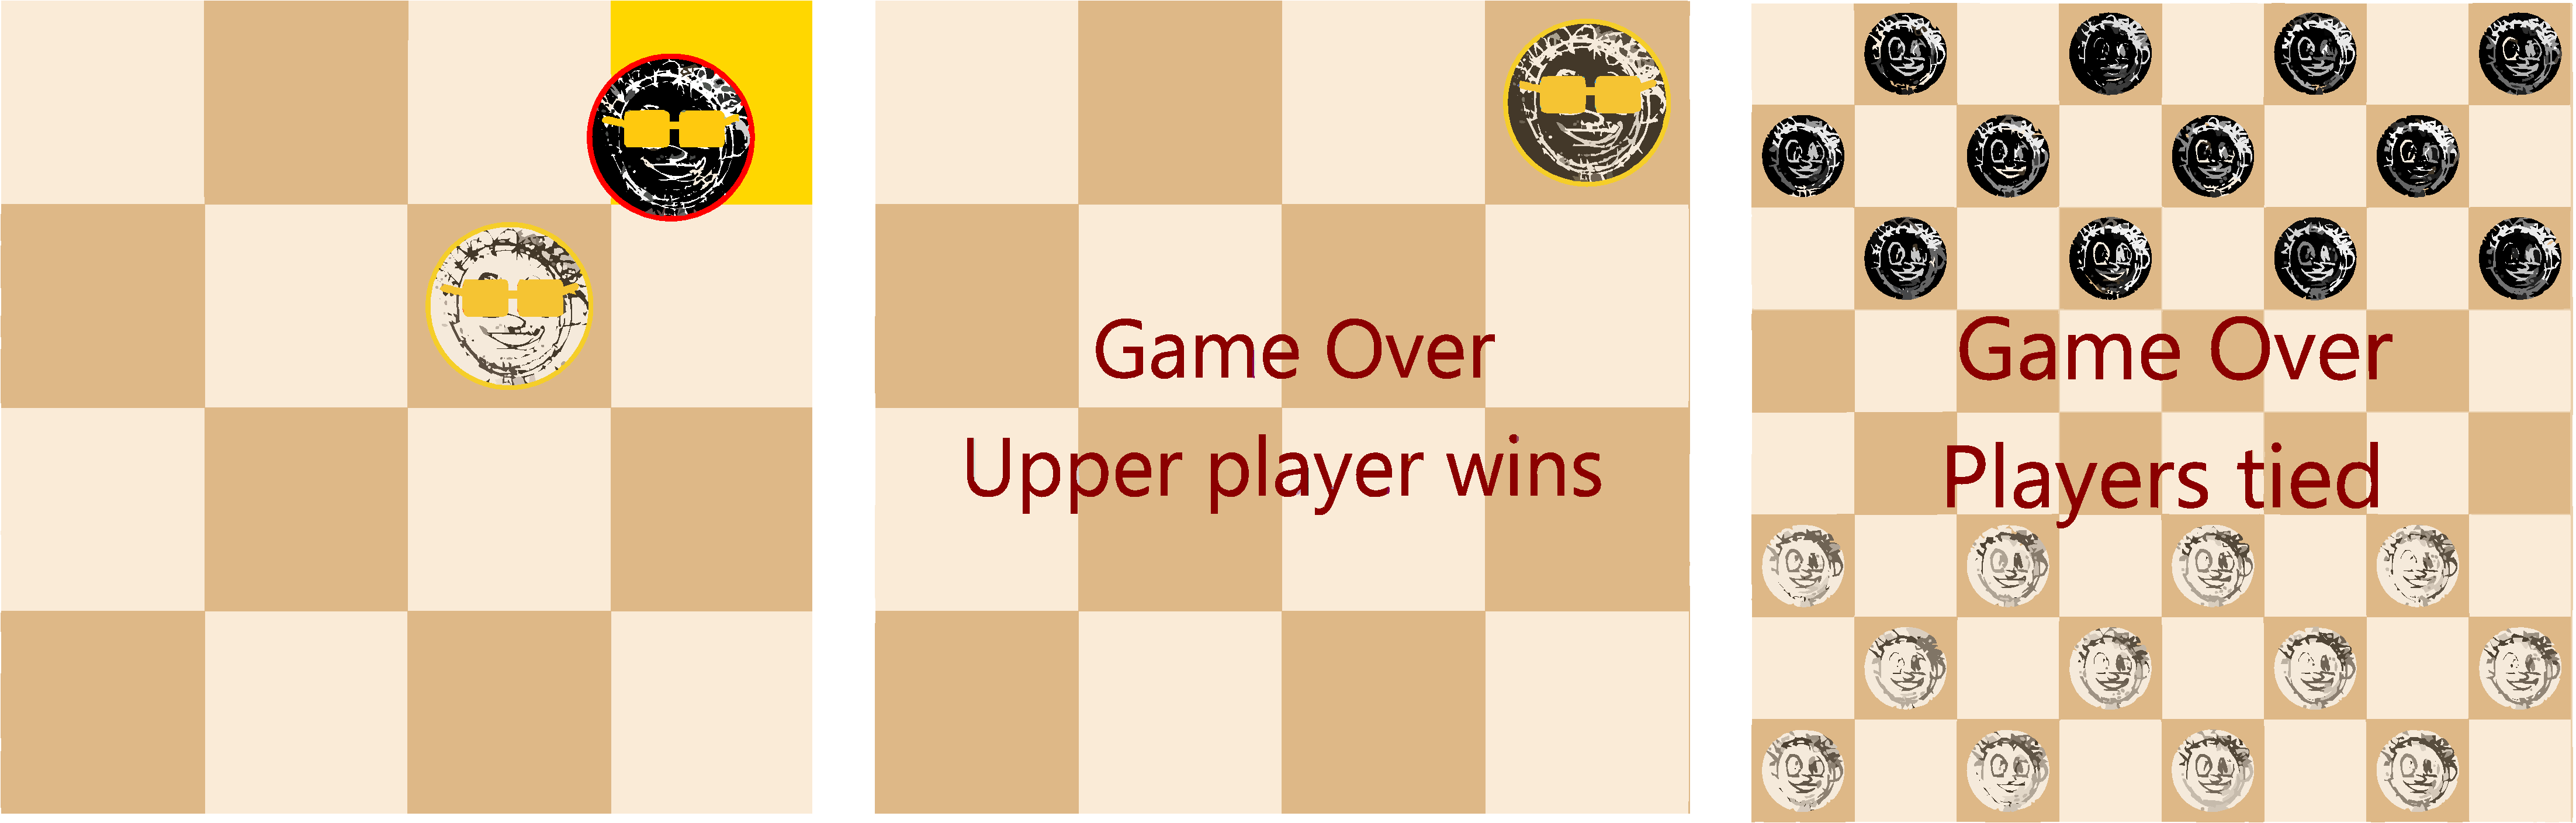
\includegraphics[width = 1.0 \textwidth]{Figurer/gameOverWinTie.pdf}
        \caption{Her kan det ses hvordan et spil afsluttes. Spillet er ovre hvis en spiller er løbet tør for brikker, hvis en spiller ikke kan flytte en brik, eller hvis begge spillere vælger at sige uafgjort spil.}
        \label{fig:gameOverWin}
    \end{figure}

\textit{Uafgjort:} I \texttt{gameScene} er der to knapper i form af \texttt{CheckBox upperTieCheckBox} og \\
\texttt{bottomTieCheckBox}. Disse har hver en listener, der, når de bliver hakket af, tjekker om begge check boxes er blevet hakket af. Hvis dette er sandt, køres metoden \texttt{gameOver}. \texttt{gameOver} laver en label, indeholdende tekst afhængig af hvordan spillet blev sluttet. Denne label bliver sat ind i \texttt{damModel}, og derefter sættes \texttt{playerThisTurn} til \texttt{None}, hvilket gør at ingen spiller kan tage deres træk. \\

%   RR
%    \item Hvordan er save og load implementeret?
%    \item Hvordan lagres data i en save file? 
%    \item Hvordan forhindres fejl loading? (load uden save file) 
\textbf{Save og load:} 
Save og load bruger hovedsageligt \texttt{Serializable} og klasserne \\
\texttt{ObjectOutputStream}/\texttt{ObjectInputStream}. Klassen \texttt{ResourceManager} håndterer selve det at gemme og hente filerne ved brug af det givne filnavn i strengen \texttt{"filename"}. Data om modellen, der skal gemmes, lagres i \texttt{ModelData}. Dvs.: de anvendte indstillinger og brikkerne på brættet. Da brikkerne nedarver \texttt{Ellipse} er de ikke \texttt{Serializable}, så de konverteres ved brug af klassen \texttt{PieceData}. \texttt{PieceData} indeholder brikkens position, spiller og om den er kronet. \\

Når brikkerne er gemt via \texttt{PieceData} og spillet er gemt i \texttt{ModelData}, gemmes det i en lokal fil med navnet \texttt{"Checkers.sv"}. Den gemte fil bliver gemt uden for \texttt{.jar} filen ved brug af klassen \texttt{ObjectOutputStream}.\\

Hver gang spillet startes bliver der tjekket om en legal gemt fil findes i samme directory hvilket bestemmer om \texttt{"Load"} knappen er aktiv eller ej. Så snart man trykker på \texttt{"Save"} vil load blive aktiv igen, da det så er sikkert at filen er legal. \\

Den eneste måde at prøve at loade en illegal fil på er ved at have spillet kørende imens man ændrer i den gemte fil, og så prøve at loade den. På den måde er filen ikke blevet tjekket inden den hentes, men vil da blive fanget i en \texttt{try-catch} og stoppet. Hvis man prøver at hente illegal en fil, vil knappen \texttt{"Load"} kunne klikkes, men den vil ikke gøre noget; fejlen fanges med en \texttt{try-catch}.